
%@metapost:4espaceexo32.mp
%@Auteur:Véronique Glaçon
Cet exercice est un questionnaire à choix multiples (QCM).
\\{\em Aucune justification n'est demandée.}
\\Pour chacune des questions, trois réponses sont proposées, une seule est exacte.\\
\textbf{\em Pour chacune des trois questions, indique sur la copie le numéro de la question et recopie la réponse exacte.}
\begin{center}
\begin{tabular}{|p{10cm}|c|c|c|}
 \hline     & Réponse A & Réponse B & Réponse C \\
 \hline \textbf{a)} \raisebox{-1.5cm}{\hbox{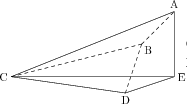
\includegraphics[scale=1]{RepS-21.png} }}\begin{minipage}{3.5cm} Cette pyramide a pour base \ldots\end{minipage}
           & $CDE$ & $ABDE$ & $ABC$ \\ 
 \hline \textbf{b)} Une pyramide dont la base à cinq côtés a : 
           & $6$ arêtes & $10$ arêtes & $15$ arêtes \\
 \hline \textbf{c)} \raisebox{-1.75cm}{\hbox{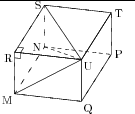
\includegraphics[scale=1]{RepS-21b.png}}}\kern5mm\begin{minipage}{5cm} La hauteur de la pyramide $UMRSN$ est :\end{minipage}
           & $[RS]$ & $[RM]$ & $[RU]$ \\
  \hline         
\end{tabular}
\end{center} 